%!TEX root = main.tex

\section{Symbolic Computation Essentials}

\begin{frame}{Symbolic Computation Essentials}{Introduction}
  \begin{itemize}
    \item Symbolic computation involves manipulating mathematical expressions in their \textbf{exact} form.
    \item Even if the size of the output is small, the intermediate expressions generated during a computation may grow unpredictably \dots
  \end{itemize}
  \hic{Expression Swell}
  \begin{center}\begin{minipage}{\textwidth}\begin{bbox}[The Ideal Workflow]
    \centering%
    \begin{minipage}[c]{0.15\textwidth} \centering Input expression \end{minipage}%
    \begin{minipage}[c]{0.19\textwidth} \centering $\autorightarrow{\text{symbolic}}{\text{manipulation}}$ \end{minipage}%
    \begin{minipage}[c]{0.21\textwidth} \centering Output expression \\ + \\ Expression swell \end{minipage}%
    \begin{minipage}[c]{0.19\textwidth} \centering $\autorightarrow{\text{symbolic}}{\text{simplification}}$ \end{minipage}%
    \begin{minipage}[c]{0.21\textwidth} \centering Output expression \\ + \\ \xout{Expression swell} \end{minipage}%
  \end{bbox}\end{minipage}\end{center}
  \hic{All \acp{CAS} are sensitive to expression swell, some more than others!}
\end{frame}

\subsection{Expression Swell}

\begin{frame}{Expression Swell}{A Rough Definition}
  \begin{bbox}[Not-So-Formal Definition]
    Exponential growth of expression size during symbolic manipulation, which undermines \ac{CAS} efficiency and leads to high memory usage and slow computation.
  \end{bbox}
  \vspace{0.75em}
  There are two types of expression swell \dots
  \vspace{0.75em}
  \begin{columns}
    \begin{column}[t]{0.5\textwidth}
      \hi{\large Inherent \textcolor{black}{expression swell}} \\
      \begin{itemize}\small
        \item Size of expressions can not be lowered due to no simplification rules being applicable.
        \item Can not be avoided and requires changes in the problem formulation.
      \end{itemize}
    \end{column}
    \begin{column}[t]{0.5\textwidth}
      \hi{\large Intermediate \textcolor{black}{expression swell}} \\
      \begin{itemize}\small
        \item During the middle stages of a calculation the size of intermediate expressions can expand substantially \emph{en route} to a comparatively simple final result.
        \item Strongly tied to the \ac{CAS}'s simplification capabilities.
      \end{itemize}
    \end{column}
  \end{columns}
\end{frame}

\subsection{\acl{LEM}}

\begin{frame}{\acl{LEM}}{Hierarchical Representation}
  The \textbf{hierarchical representation} of expressions is carried out through \textbf{veiling variables}, which are defined as \dots
  \begin{equation*}
    \m{f}(\mx) \quad \autorightarrow{\text{veiling}}{\text{variables}} \quad \m{f}(\mx, \m{v})
    \qquad \text{where} \qquad
    \m{v}(\mx) = \msmall{\begin{bmatrix}
      v_{1}(\mx) \\
      v_{2}(v_{1}, \mx) \\
      \vdots \\
      v_{n}(v_{1}, \dots, v_{n-1}, \mx)
    \end{bmatrix}}
  \end{equation*}
  The process is composed of two actions \dots
  \begin{enumerate}
    \item a large expression can be \textbf{veiled} (stored) in a \textbf{veiling variable};
    \item veiling variables can be \textbf{unveiled} (substitute back) the veiling variables into the expression to recover the original form.
  \end{enumerate}
  \vspace{0.5em}
  \hic{The complexity remains but the \ac{CAS} can not see it! \raisebox{-2.5pt}{\Huge\trollface{}}}
\end{frame}

\begin{frame}{\acl{LEM}}{An Example of \acs{LEM} through Hierarchical Representation}
  Let us consider an expression of the form
  \begin{equation*}
    \textcolor{mycolor1}{\underline{2xy(1+y)}} \cdot f(x,y) +
    \textcolor{mycolor2}{\underline{5z(3a+z)}} \cdot g(y) +
    \textcolor{mycolor3}{\underline{3c(xy+z)}} \cdot h(x,z) \text{.}
  \end{equation*}
  One of its possible hierarchical representations is
  \begin{equation*}
    \textcolor{mycolor1}{v_1} \cdot f(x,y) +
    \textcolor{mycolor2}{v_2} \cdot g(y) +
    \textcolor{mycolor3}{v_3} \cdot h(x,z) \text{,}
  \end{equation*}
  where the veiling variables are
  \begin{equation*}
    \textcolor{mycolor1}{v_1} = 2x(1+y) \text{,}
    \qquad
    \textcolor{mycolor2}{v_2} = 5z(3a+z) \text{,}
    \qquad \text{and} \qquad
    \textcolor{mycolor3}{v_3} = 3c(xy+z) \text{.}
  \end{equation*}
\end{frame}

\begin{frame}{\acl{LEM}}{Measuring Expression Complexity}
  Easy to implement, but \dots
  \vspace{1.5em}
  \begin{columns}
    \begin{column}[t]{0.5\textwidth}
      \hi{\large How to measure symbolic expression complexity?}
      \begin{itemize}
        \normalsize
        \item \textbf{Length in characters}: already used by other authors, not reliable;
        \item \textbf{Directed acyclic graph}: measures the number of nodes and edges.
        \item \textbf{Computational cost}: insensible to expression internal representation. \\[0.25em]
        \emph{We can roughly predict the swelling related to elementary mathematical operations!}
      \end{itemize}
    \end{column}
    \begin{column}[t]{0.5\textwidth}
      \hi{\large How to choose the right level of expression complexity?}
      \begin{itemize}
        \normalsize
        \item \textbf{Prediction}: based on the specific operations to be performed;
        \item \textbf{Trial and error}: no general rule, depends on the software.
      \end{itemize}
    \end{column}
  \end{columns}
\end{frame}

\begin{frame}{\acl{LEM}}{The \ac{LEM} Package}
  \Maple{} package for managing large symbolic expressions \dots
  \begin{itemize}
    \item \textbf{custom implementation} of the \Maple{}s' \texttt{LargeExpressions} package.
    \item \textbf{object-oriented} implementation for managing large symbolic expressions;
    \item \textbf{better control} over the hierarchical representation of expressions.
  \end{itemize}
  %
  \begin{bbox}[Large Expression Management \Maple{} package]
    The LEM implementation is freely available on GitHub! \\
    \centering \url{https://github.com/StoccoDavide/LEM}
  \end{bbox}
\end{frame}

\subsection{Symbolic Matrix Factorization}

\begin{frame}{Symbolic Matrix Factorization}
  \textbf{Numeric} factorization is a fundamental operation in numerical linear algebra. It is used to \dots
  \begin{itemize}
    \item solve linear systems of equations without inverting the original matrix;
    \item reduce the number of computations and increase the stability;
    \item provide insights into the properties of the original matrix (\ie{}, rank and determinant).
  \end{itemize}
  \vspace{1.0em}
  \hic{Does this also apply to the symbolic computation? Yes!}
  \vspace{1.0em}
  However\dots
  \begin{enumerate}
    \item the output is not guaranteed to be stable once numerically evaluated;
    \begin{itemize}
      \item[] \textbf{How to ensure the stability of the symbolic factorization?}
    \end{itemize}
    \item symbolic expressions tend to grow during manipulation.
    \begin{itemize}
      \item[] \textbf{How to manage large symbolic expressions?}
    \end{itemize}
  \end{enumerate}
\end{frame}

\begin{frame}{Symbolic Matrix Factorization}
  \begin{itemize}
    \item There are a multitude of matrix factorizations, we choose \textbf{\ac{LU}} and \textbf{\ac{FFLU}} because of \dots
    \begin{enumerate}
      \item capability of preserving \textbf{sparsity} with \textbf{minimum degree} approach;
      \item limited expression swell with the \textbf{full-pivoting} strategy;
      \item improved numerical stability with custom symbolic \textbf{pivoting strategy};
      \item depending on the formulation, improved numerical stability with \textbf{fraction-free} factorization.
    \end{enumerate}
    \item \Maple{} matrix factorizations are \textbf{sensitive to expression swell}.
    \item We developed a symbolic matrix factorization toolbox capable of dealing with expression swell.
    \begin{enumerate}
      \item At specific steps of the algorithm \textbf{veiling variables} are introduced not to increase the size of the expressions.
    \end{enumerate}
\end{itemize}
  %
  \begin{bbox}[Linear Algebra Symbolic Toolbox \Maple{} package]
  The LAST object-oriented implementation is freely available on GitHub! \\
  \centering \url{https://github.com/StoccoDavide/LAST}
\end{bbox}
\end{frame}

\begin{frame}{Symbolic Matrix Factorization}{Pivoting Strategy}
  \hic{How to ensure the stability of the symbolic factorization? \\
  \textcolor{black}{With a good pivoting strategy!}}
  \begin{columns}
    \begin{column}[c]{0.5\textwidth}
      A good pivoting strategy should \dots
      \begin{itemize}
        \item select the simplest pivot element;
        \item[] \textbf{\small Avoid excessive expression swell}
        \item select the pivot element to ensure numerical stability;
        \item[] \textbf{\small Avoid numerical instability}
        \item explore all the possible pivots to make the best choice.
        \item[] \textbf{\small Avoid numerical errors}
      \end{itemize}
    \end{column}
    \begin{column}[c]{0.5\textwidth}
      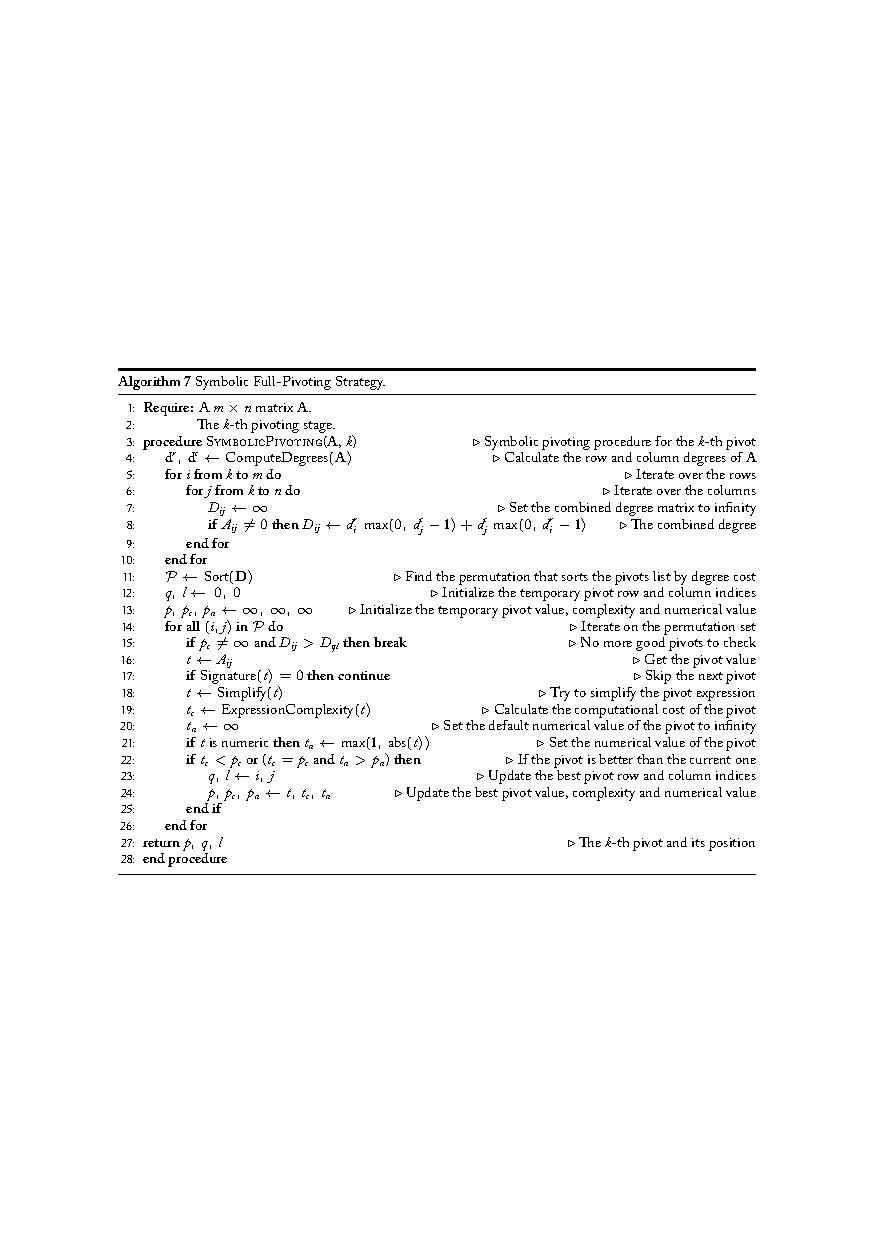
\includegraphics[width=\textwidth]{pivoting_strategy}
    \end{column}
  \end{columns}
\end{frame}

\begin{frame}{Symbolic Matrix Factorization}{\ac{LEM} During Factorization}
  \hic{How to manage large symbolic expressions? \\
  \textcolor{black}{By using \ac{LEM} during the factorization!}}
  Veiling variables are introduced during \dots \\[1.0em]
  \begin{columns}
    \begin{column}[t]{0.5\textwidth}
      \textbf{Factorization step} \\
      \begin{itemize}\small
        \item Gaussian elimination;
        \item Schur complement computation.
      \end{itemize}
      {\centering 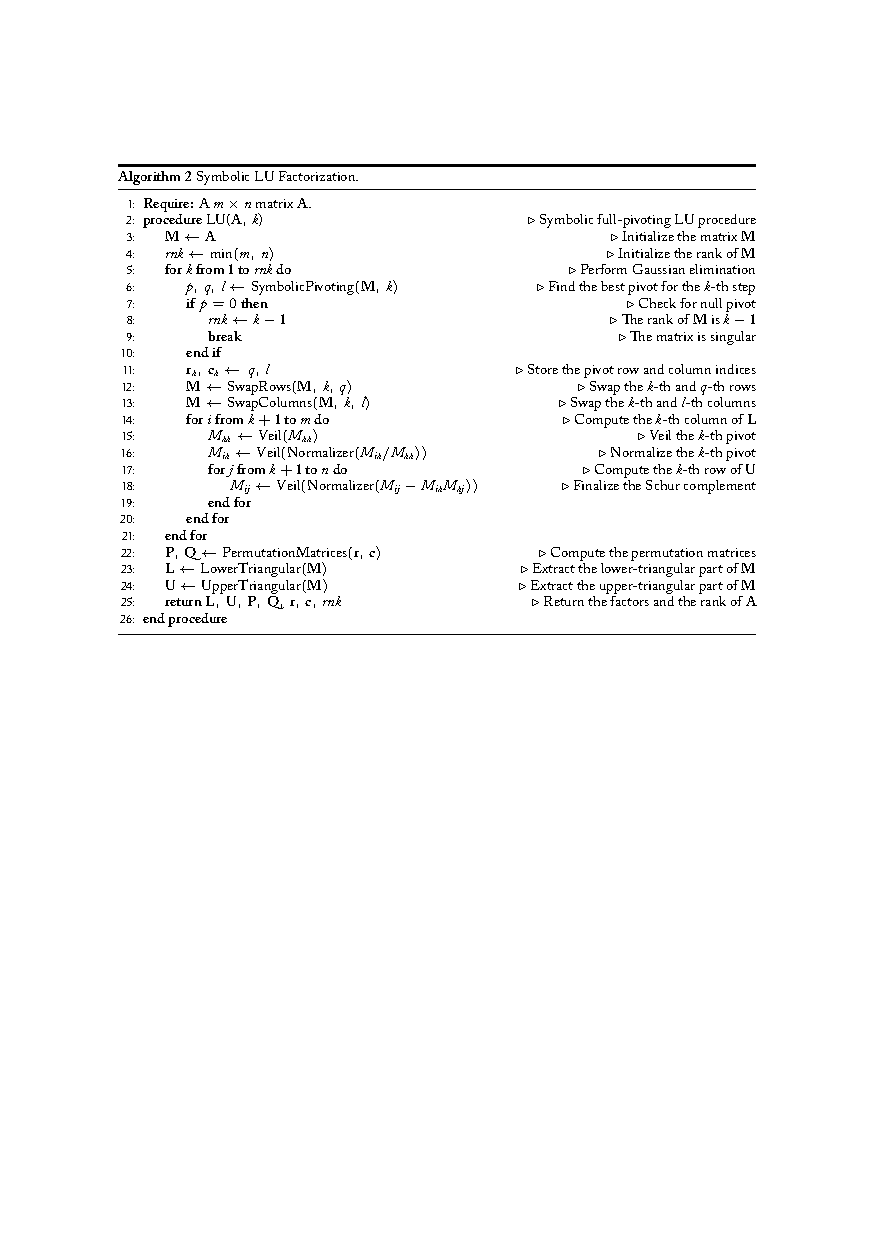
\includegraphics[width=\textwidth]{factorization_lu}}
    \end{column}
    \begin{column}[t]{0.5\textwidth}
      \textbf{Solution step} \\
      \begin{itemize}\small
        \item Forward substitution;
        \item Backward substitution.
      \end{itemize}
      {\centering 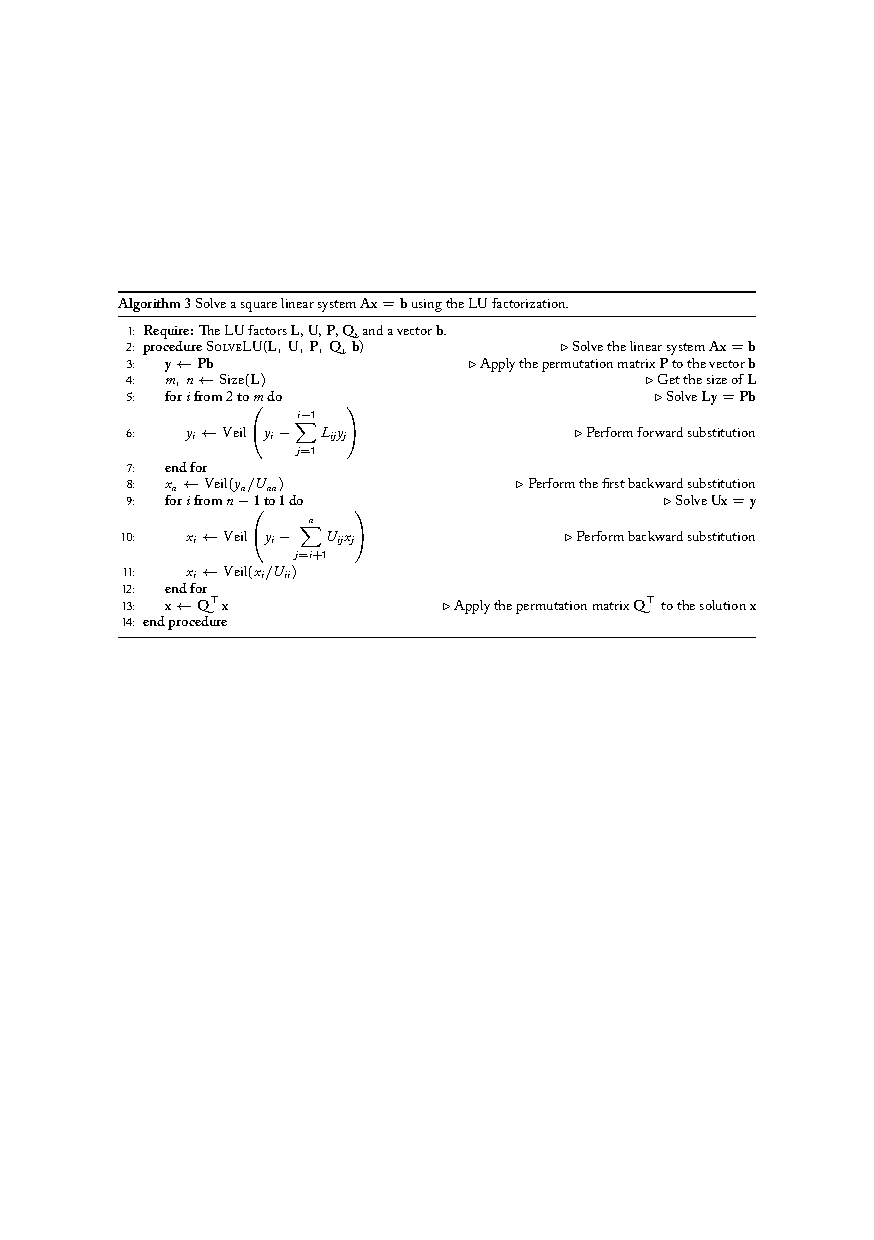
\includegraphics[width=\textwidth]{solve_lu}}
    \end{column}
  \end{columns}
\end{frame}

% That's all Folks!
